% neginhib cogsci submission


\documentclass[10pt,letterpaper]{article}

\usepackage{cogsci}
\usepackage{pslatex}
\usepackage{apacite}
\usepackage{graphicx}

\usepackage{color}
 \newcommand{\denote}[1]{\mbox{ $[\![ #1 ]\!]$}}
 \definecolor{Red}{RGB}{255,0,0}
\newcommand{\red}[1]{\textcolor{Red}{#1}}
\definecolor{Green}{RGB}{10,200,100}
\definecolor{Blue}{RGB}{10,100,200}
\definecolor{DarkOrange}{RGB}{255,100,50}
\newcommand{\ejy}[1]{\textcolor{Blue}{[ejy: #1]}} 
\newcommand{\aen}[1]{\textcolor{DarkOrange}{[aen: #1]}}  
\newcommand{\gabe}[1]{\textcolor{Green}{[gabe: #1]}}  



\title{Distinct mechanisms of linguistic and non-linguistic inference in preschool children}
 
\author{{\large \bf Ann E. Nordmeyer} \\
  \texttt{anordmey@stanford.edu} \\
  Department of Psychology \\
  Stanford University
  \And {\large \bf Erica J. Yoon} \\
  \texttt{ejyoon@stanford.edu} \\
  Department of Psychology \\
  Stanford University
  \And {\large \bf Michael C. Frank} \\
  \texttt{mcfrank@stanford.edu} \\
  Department of Psychology \\
  Stanford University}

\begin{document}

\maketitle


\begin{abstract}

...

\textbf{Keywords:} 
Inhibitory control; negation; implicature; drift diffusion model; cognitive development; pragmatics

\end{abstract}


\section{Introduction}
Children often fail traditional language processing tasks that test important but complex linguistic constructions.  For example, children in a forced-choice task will often struggle to identify a character who ``doesn't have apples'', instead choosing the character who \emph{does} have apples \cite{nordmeyer2014b}.  And while adults easily make the inference that ``My plate has a carrot'' refers to a plate with \emph{just} a carrot, not a plate with a carrot and a banana, children struggle to make this choice \cite{yoonchildren}.   Although these two examples, negation and pragmatic implicatures, are very different linguistic phenomenon, comprehension on both tests requires children to resist choosing a more salient (but incorrect) alternative.  Could poor inhibitory control account for children's difficulty on both of these tasks?

A pragmatic implicature \cite{grice1975} is made when a listener makes an inference about a speaker's intended meaning that goes beyond the literal meaning of an utterance.  For example, when people hear a sentence such as ``My friend has glasses'' in a context where there is a person with only glasses and a person with a hat \emph{and} glasses, people assume that the sentence refers to the person with just glasses, because if you had meant the person with a hat you would have said so.  This type of implicature is called an \emph{ad-hoc} implicature, because the inference depends on context (as opposed to e.g. scalar implicatures, which rely on knowledge of specific lexical scales).  Children up to three years of age can struggle to make ad-hoc implicatures (\citeNP{yoonchildren}, though c.f. \citeNP{stiller2014}) as well as scalar implicatures \cite{huang2009}.  Children's difficulties on these tasks is surprising, because children demonstrate an understanding of pragmatic principles from an early age \cite<e.g.>{katsos2011pragmatic, matthews2012tw}.  \aen{This last sentence could probably use a little bit of expansion, it feels weak right now -- Erica, could you take a stab at making this point a little stronger? }

Children's difficulty on tests of negation comprehension is also unexpected given children's early production of negative sentences.  Children spontaneously produce denial negation before their second birthday in both natural \cite{bloom1970, pea1980} and experimental contexts \cite{pea1982}.  Despite this, children as old as four years consistently fail on classic tests of negation comprehension \cite<e.g.>{kim1985, nordmeyer2014b}.  For example, children will look at a picture of a character \emph{with} apples when told to look at the boy with \emph{no} apples, and will rate a puppet's true negative utterance (e.g. ``this is not an apple'', when describing a picture of a banana) as ``silly'' or ``wrong''. If children's production of negative sentences suggests that even two-year-olds have the linguistic knowledge of how negative words work, then children's performance on these tasks may reflect processing difficulties rather than a true lack of comprehension.  

Why do children struggle on these language comprehension tasks when production data and past experiments suggest that they have the requisite linguistic abilities? In both of these examples, children's failures might occur not because they lack linguistic understanding, but because the incorrect choice is more salient or perceptually interesting.  For example, when a child is asked to ``find the boy with no apples'', she must look \emph{away} from the character who is holding the labeled objects, and look at some other, unlabeled object instead.  Similarly, to demonstrate comprehension of an ad-hoc implicature, such as ``my plate has a carrot'' referring to a plate with just a carrot instead of a plate with a carrot and a banana, children must look away from the more interesting plate (i.e. the plate with two objects instead of one) to demonstrate understanding of the implicature.  In both of these cases, poor inhibitory control might explain children's difficulty executing the correct response on these comprehension tasks.  Inhibitory control is a broad construct that encompasses a wide variety of different functions \cite{miyake2000} and changes dramatically during early childhood \cite{diamond1996,davidson2006}. We hypothesized that preschool children's poor inhibitory control, rather than undeveloped semantic or pragmatic knowledge, can account for children's failure on negation and implicature comprehension tasks.

Classic tests of inhibitory control require participants to override a prepotent response. Participants who react quickly often make the wrong choice, and correct choices are typically slower.  This speed-accuracy tradeoff can be difficult to understand with traditional analyses, which examine reaction time and accuracy separately.  
The drift diffusion model \cite<e.g.>{ratcliff1978theory} uses both accuracy and reaction time to model the decision making process in simple two-alternative forced choice paradigms.  The model can be imagined as a noisy accumulation of evidence over time, resulting in an eventual correct or incorrect choice when the accumulated evidence reaches a predetermined ``boundary''.  The model produces four key parameters: boundary separation (the amount of evidence needed to reach a positive decision), bias (to what extent is the decision process biased towards one decision or another), non-decision time (the time needed to encode basic information about the stimuli, before embarking on the decision process), and drift rate (the rate at which evidence is accumulated).  Past work has shown that children typically have longer non-decision times, higher separation boundaries, and slower drift rates, suggesting that children require more time to process stimuli, more information to make a decision, and take longer to accumulate evidence compared to adults \cite{ratcliff2012}. In this study, we use the drift diffusion model to explore whether children's negation and implicature processing resembles their decision-making process on a similar test of inhibitory control.  

In the current study, we use a simple game with three phases to test adults' and children's inhibitory control, negation comprehension, and implicature comprehension.  In order to explore how children's language processing changes across development, we collected data from four-year-olds, five-year-olds, and six-year-olds, as well as adults.  Despite the fact that the three tasks contained almost identical visual and auditory stimuli, we found distinct patterns of information processing and developmental change across the three games.  This suggests that, contrary to our hypothesis, children's poor inhibitory control cannot entirely explain their difficulty with negation and pragmatic implicatures, and children's development of negation and implicature appear to follow different developmental trajectories throughout early childhood. 

\section{Method}

In pilot work, we used a classic ``find the picture'' comprehension task to explore whether 4-year-old children's difficulty processing implicatures and negation might be due to poor inhibitory control.  Our hypothesis was that undeveloped inhibitory control could lead children to quickly choose the more salient incorrect choice rather than selecting the answer they know to be correct.  Although we did not find any correlation between children's inhibitory control processing and their negation or implicature processing, we found that this simple comprehension task was even more challenging for 4-year-olds than our past work has indicated, with 4-year-olds barely exceeding chance performance on negation and implicature trials.  Surprisingly, we found no reaction time differences between 4-year-olds responses to negation/implicature trials and control trials. In our extension of this pilot data we modeled children's responses using the drift diffusion model, which can help us understand the process that leads children to make so many errors on these tasks.  

\subsection{Participants}

We invited parents and children (N = 100) at the Children's Discovery Museum in San Jose, CA to play a computer game.  Ten children whose parents indicated that they hear English at home 50\% of the time or less were excluded from analysis.  An additional 24 children were excluded from analysis for failing to complete at least half of the trials in each game.  This resulted in a final sample of 22 4-year-olds (mean age 4;7), 19 5-year-olds (mean age 5;5), and 25 6-year-olds (mean age 6;5).  We also recruited adult participants (N = 50) on Amazon Mechanical Turk to play the computer version of the task.  Two adults were excluded for failing to complete at least half of the trials in each game, resulting in a final sample of 48 adults.  

\subsection{Stimuli and Design}

The game consisted of three phases that each tested one of the target processes: inhibition, negation processing, and implicature processing.  In each trial in all three phases, there were two images side-by-side on the screen. A pre-recorded voice said one or two words \ejy{should we justify why we decided to use 1-2 words instead of a whole sentences used in traditional tasks?} to refer to one of the images, and participants' task was to select the correct referent as soon as they could identify it.

For the ``inhibition'' phase, in a set of 6-8 trials, the same two pictures appeared side-by-side (e.g., a picture of a carrot and a picture of a banana), with randomized sides. For the first 5-7 trials (control trials), one of the two objects was named (e.g., ``carrot''), then on the last trial  (target trials), the other object was named (``banana''). Participants were predicted to become increasingly accustomed to choosing the carrot in control trials and thus gain speed. Then in the target trial, when they need to switch and choose the banana, the speed of reaction and accuracy rate were predicted to fall due to the inhibitory demand. Child participants saw a total of 12 sets of trials, and adults saw 24 sets, in the inhibition phase.

For the ``negation'' phase, the referents were named with or without negation. For example, given two pictures of carrot and banana respectively, to refer to the banana the recorded voice said ``banana'' (i.e. positive trials, the control for this phase) or ``no carrot'' (i.e. negative trials, the target for this phase). Children saw 60 trials, and adults saw 120 trials in the negation phase. 

For the ``implicature'' phase, in each trial there was a picture with one object (e.g., carrot) and another picture with the same object and another one (e.g., carrot and banana). In control trials, the unique object was named (``banana'') and in target trials, the common object was named (``carrot''), implying ``carrot \emph{but not banana}'' (i.e. ad-hoc implicature). Children saw 60 trials, and adults saw 120 trials in the implicature phase.  

\subsection{Procedure}

For child participants, an experimenter first explained the game.  Children then went through two practice trials, where they were asked to select an obvious, unambiguous referent (e.g., ``cow'' as opposed to ``rabbit'').  Children selected the picture on the left side of the screen by pressing the `z' key and selected by picture on the right side of the screen by pressing the `/' key; both keys were covered by blue stickers to help children find the correct keys. Then they went through the three test phases in a randomized order.  After the child participants were finished, the experimenter gave them a sticker as a gift and thanked them for playing the game.

Adult participants played the same game without practice trials.  Instructions indicated that participants should select the picture on the right by pressing the `p' key and select the picture on the left by pressing the `q' key.  

\section{Results and Discussion}

organize by claims
- kids aren't good at this (accuracy), no individual correlations between performance on one game and another
- due to speed-accuracy tradeoffs (which might be different for different games), we look at DDM
	- this also indicates different processes (adults)
	- Development of these processes is different, too: 
	implicature: kids get faster overall (i.e. control trials) but less for targets (becaues they are ambiguous)
	negation: kids get faster on target trials (i.e. they are struggling on negation specifically)
	So kids look like they are just bad at both, but they are bad for different reasons that the DDM can tease 	apart.

\aen{I'm concerned by how much space the results take up (the reaction time \& accuracy results added an entire page), and how easy it is to get bogged down in a zillion statistics.  I've tried to start each section with an overview of what is going on, and end each section with a little discussion/explanatory sentence/paragraph, but I'm still worried that the actual reported statistics are really overwhelming}
\ejy{Echoing your concern, Ann, one additional page of results for accuracy and RT does seem a little long, it feels like this section is taking away too much attention away from the next section which is our real focus... Is it possible to include a table of stats for accuracy and RT and write out only the key findings, especially surprising ones that led us to pursue DDM?}

For our analyses, because some children responded immediately without listening to the entire word and some children took an exceedingly long time to respond to some trials, we made a post-hoc decision to remove any trials with reaction times less than 200 milliseconds from the word onset, and longer than 15 seconds from the word onset.\footnote{Although this was a post-hoc decision based on some unexpectedly short and long reaction times, this decision did not effect the key findings we present in this paper.}  In addition, in accordance to our planned analysis, we removed any trials where participants responded outside of three standard deviations from the mean in log space.

\subsection{Proportion Correct}

We began by looking the proportion of trials that participants answered correctly across all three games (Figure \ref{fig:traditional}).  Across all three games and all age groups, participants were more accurate on control trials (i.e. repeated trials in the inhibition game, unambiguous trials in the implicature game, and positive trials in the negation game) compared to target trials (i.e. switch trials in the inhibition game, implicature trials in the implicature game, and negative trials in the negation tame). Children's performance improves modestly from four years to six years, with adults at near-ceiling performance.  

We fit two generalized linear mixed-effects models, with subject ID as a random effect, to the data for each game to test the reliability of these developmental patterns.  First, to compare children's performance to adults' performance, we effect-coded age to bin all three age groups together.  In the inhibition game and the implicatures game, we found main effects of trial type (inhibition: $\beta = -2.10$, $p< .001$; implicatures: $\beta = -1.15$, $p< .001$) and age group (inhibition: $\beta = -1.45$, $p< .001$; implicatures: $\beta = -.95$, $p< .001$), indicating that participants in these two games were much more likely to answer incorrectly on target trials compared to control trials, and with children having a much lower proportion correct compared to adults. These main effects were not significant for the negation game.  In the inhibition game, a significant \emph{positive} interaction between age group and trial type indicates that the difference in accuracy between age group and trial type is actually smaller for children compared to adults ($\beta = .63$, $p< .05$), while a \emph{negative} interaction in the negation game indicates that in the negation game the difference between target and control trials was larger for children compared to adults (negation: $\beta = -1.98$, $p< .001$).  There was no significant interaction between trial type and age group on the implicatures game.  

To explore any developmental change in accuracy between four and seven years, we fit another set of generalized linear mixed-effects models to just the children's data, treating age as a continuous variable.  In the inhibition game, this model again produced main effects of age ($\beta = .55$, $p< .05$) and trial type ($\beta = -1.98$, $p< .01$), as well as a negative interaction between age and trial type ($\beta = -.7$, $p< .001$), indicating that children get worse on target trials compared to control trials as they get older.  In the implicatures game, there was a main effect of age ($\beta = .33$, $p< .05$), indicating that children get more accurate as they get older, but there was no main effect or interaction with trial type.  On the negation game, there were no significant main effects or interactions, suggesting that older children were not significantly better than younger children on this game.

\subsection{Reaction Time}

Next we looked at participants' reaction times in response to correct trials only across the three games.  Participants appear to be slightly slower on target trials compared to control trials for the inhibition and negation game, but not the implicature game.  Unlike the accuracy data, there did not appear to be a strong interaction between age group and trial type for the reaction time data.  

To examine the reliability of these findings, we fit two linear mixed-effects models, with subject ID as a random effect, to the reaction time data for each game.  As with the accuracy data, we first effect-coded age to bin children together to compare to adults.  Across all three games, we found significant main effects of age group, with children responding significantly slower compared to adults (inhibition: $\beta = .63$, $p< .001$; implicature: $\beta = .93$, $p< .001$; negation: $\beta = .69$, $p< .001$).  In the inhibition game, there was a significant difference between target and control trials, with participants responding slower to target trials compared to control trials ( $\beta = .14$, $p< .001$), as well as an interaction between age group and trial type ($\beta = .09$, $p< .001$).  There was also a significant interaction between age group and trial type for the negation game ($\beta = .15$, $p< .001$).  These interactions indicate that on the inhibition and negation games, the difference between control and target trials is larger for kids compared to adults.  

We also fit linear mixed-effects models to just the children's data with age as a continuous variable.  We again found main effects of age on reaction time for all three games (inhibition: $\beta = -.21$, $p< .001$; implicature: $\beta = -.26$, $p< .001$; negation: $\beta = -.25$, $p< .001$).  In the negation game, we also found a significant main effect of trial type ($\beta = .69$, $p< .01$) as well as an interaction between trial type and age ($\beta = -.09$, $p< .05$), indicating that children take longer to respond to negative trials compared to positive trials on the negation game, but that this difference is reduced as children get older.  

As with our past findings \cite{yoonchildren, nordmeyer2014b} and pilot data, accuracy data indicates that children ages 4 to 6 years struggled significantly with the implicature and negation games.  Despite this, the reaction time data did not find a correspondingly large effect of reaction time on trial type, particularly for the implicature game.  With these traditional analyses, we can only speculate why children might be struggling on these games.  Because traditional reaction time analyses only explore responses to correct trials (due to the documented speed-accuracy tradeoff \aen{is there a good citation for this?}), we don't know if children are making mistakes because they are rapidly making the wrong decision, or if they are slowly and deliberately making correct decisions, but sometimes reaching the wrong conclusion.  In the next section, we fit our data to the drift diffusion model \cite{ratcliff1978theory} to model the decision process that children and adults go through on each of these games.  Our goal is to get a clearer picture of how children are processing information, and what is leading them to make so many errors on these tasks. 


\begin{figure}
\begin{center} 
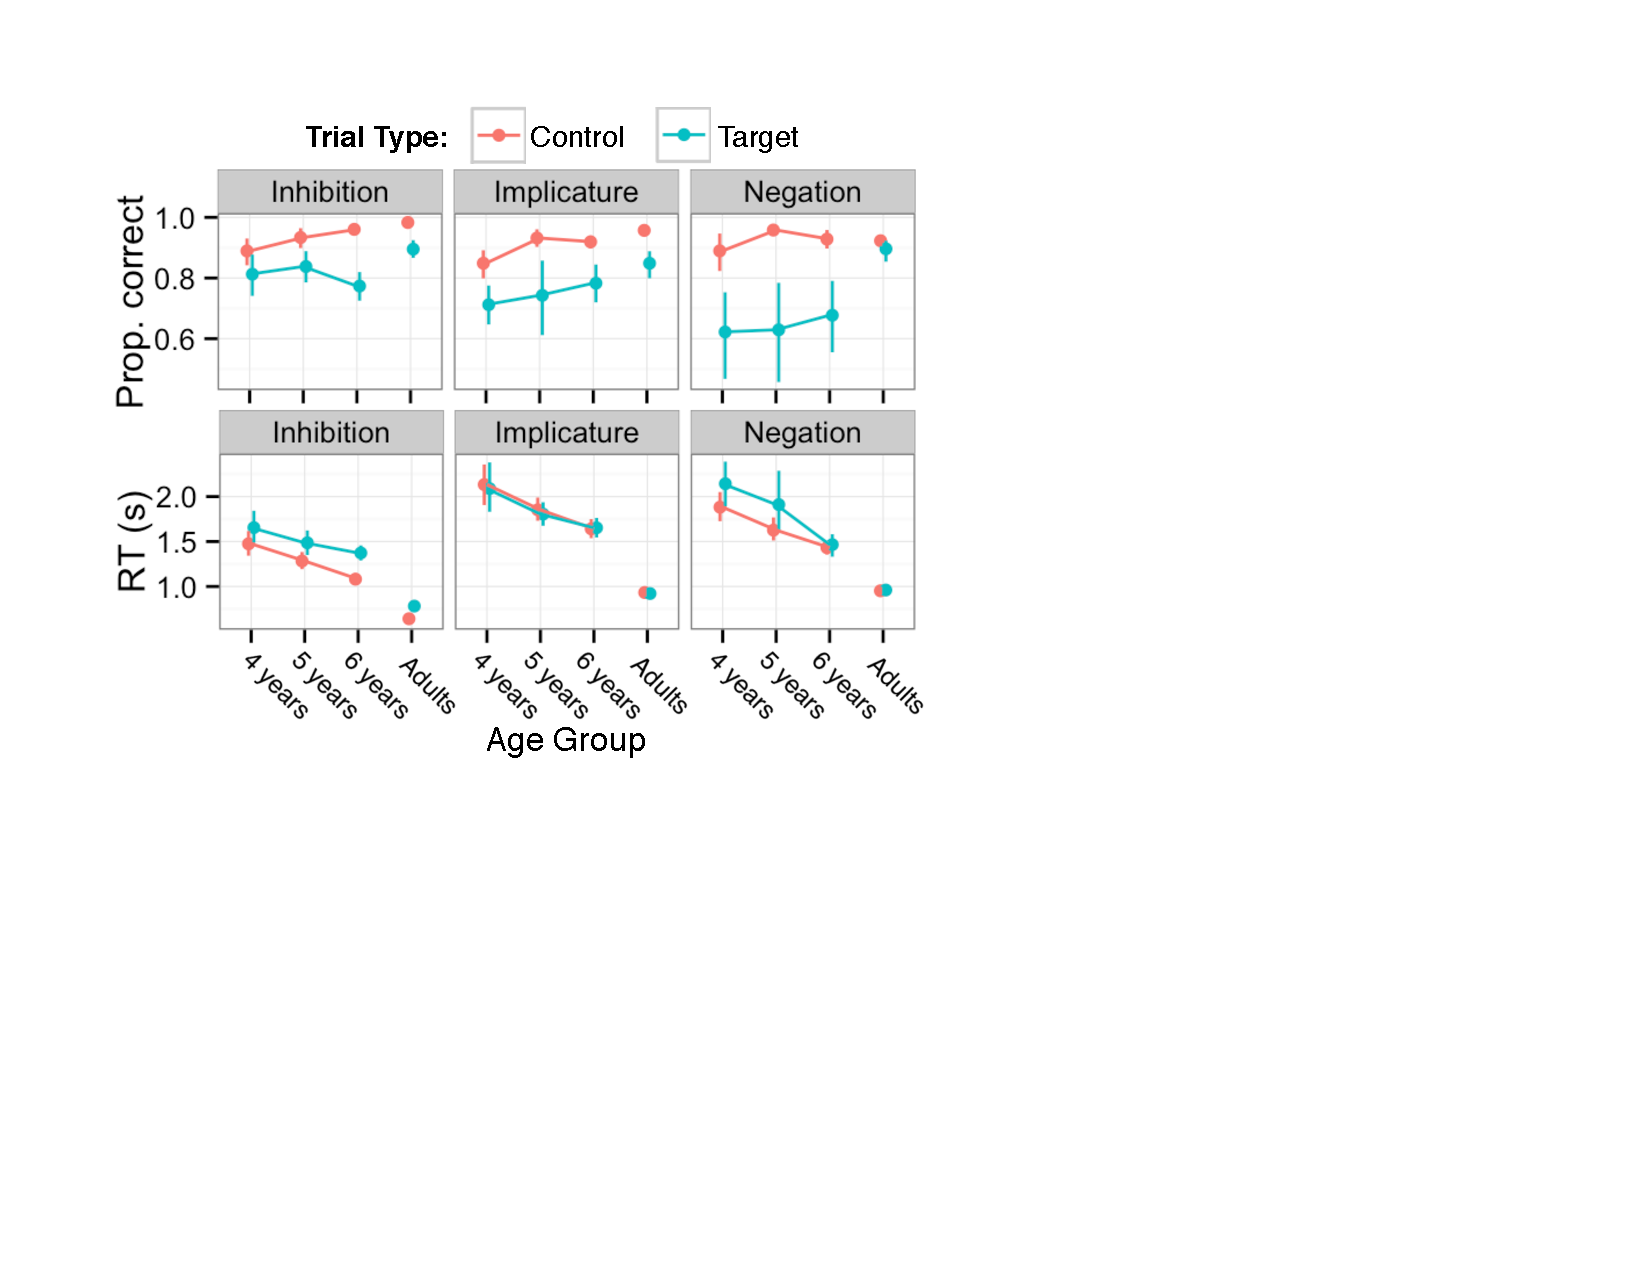
\includegraphics[width=3in]{figures/correct_RT.pdf}
\caption{\label{fig:traditional} Adults' and children's mean proportion correct responses (top) and reaction time (bottom) for target and control trials across the three games.  Control trials are shown in pink, target trials are shown in green.  Error bars show 95\% confidence intervals.  }
\end{center} 
\end{figure}

\subsection{Diffusion Analysis}

We fit the diffusion model separately to each individual participant's data using the RWiener package\footnote{All analyses described in this paper were conducted using R version 3.2.1}, which uses the Nelder-Mead method to estimate optimal parameter values.  We estimated parameters separately for each trial type (target vs. control) within each game, and calculated the mean and 95\% C.I. across all participants within each age group (4-year-olds, 5-year-olds, 6-year-olds, and adults).  We then used these parameter estimates to produce visualizations of the average decision process for each trial type across each game and age group (see Figures \ref{fig:adults} and \ref{fig:kids}).  

\subsubsection{Adults}

\begin{figure*}
\begin{center} 
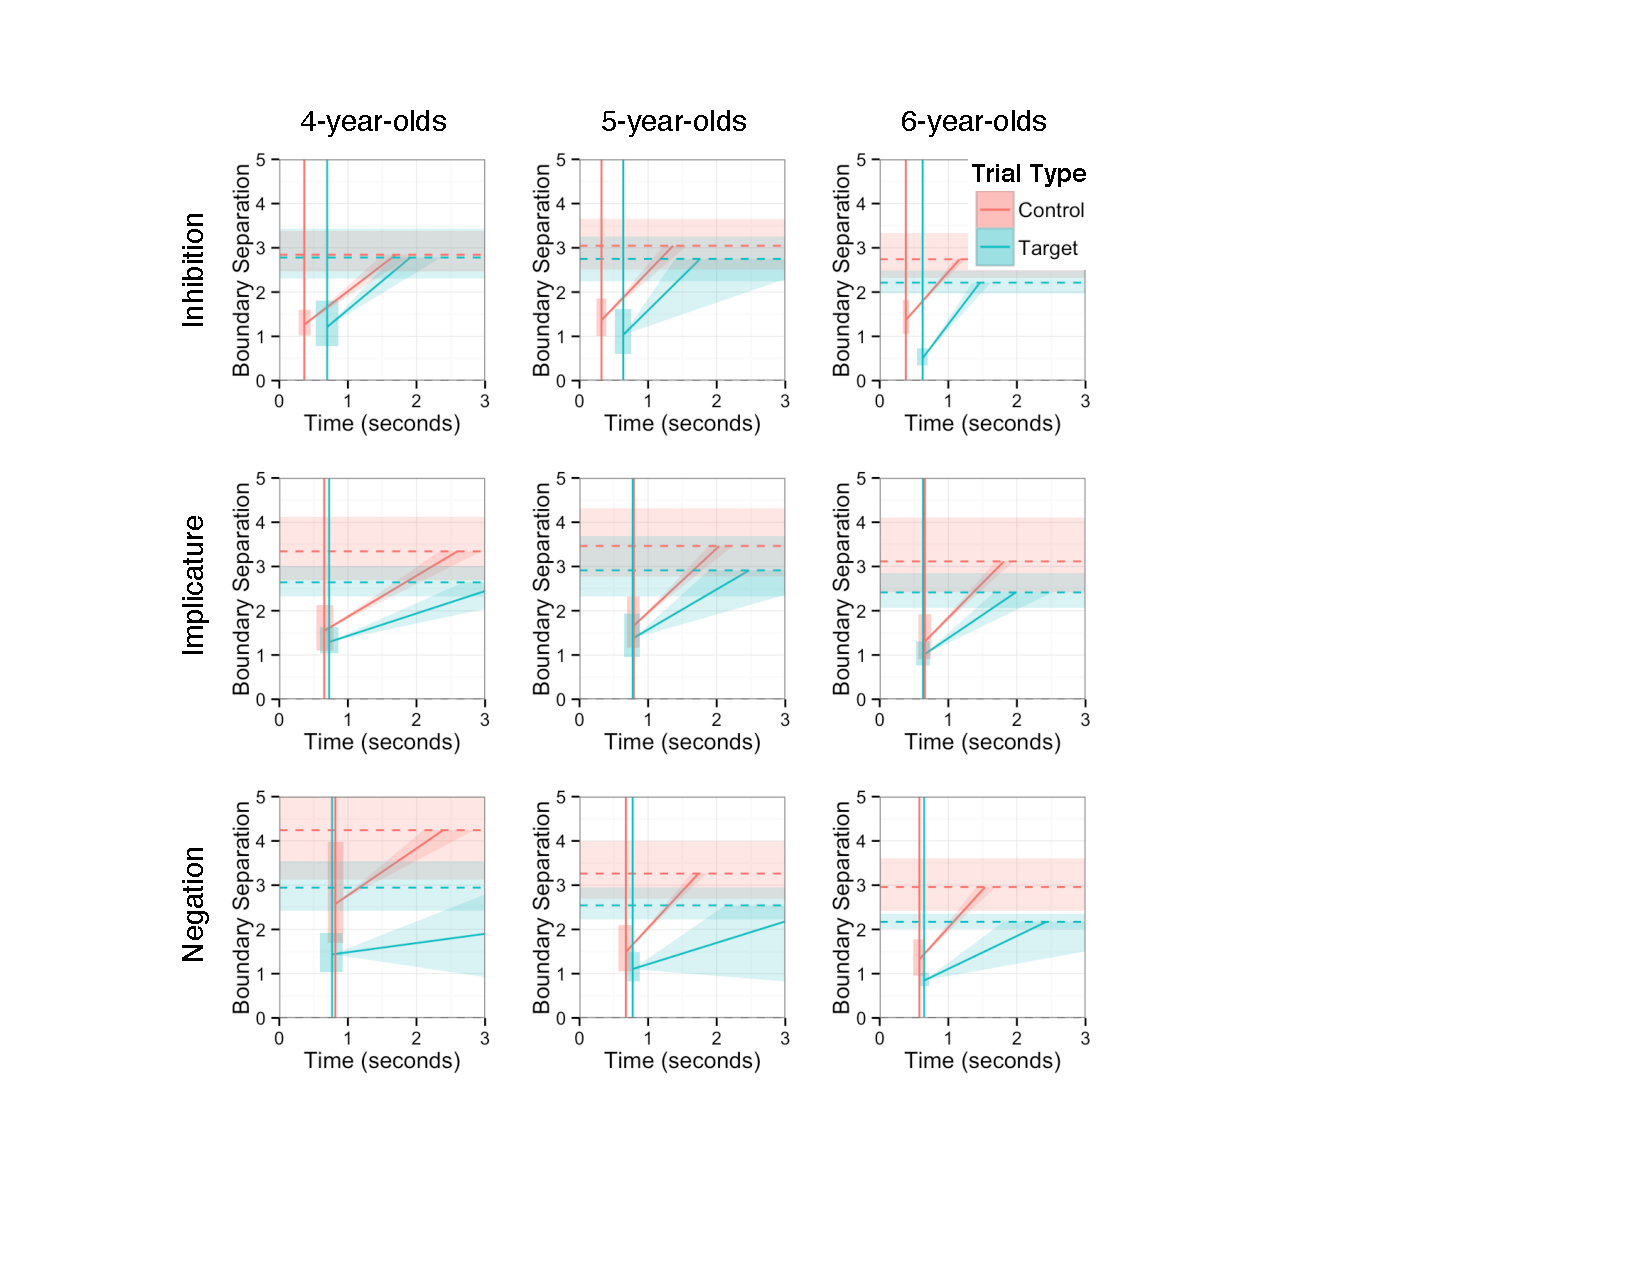
\includegraphics[width=6in]{figures/adult_vis.pdf}
\caption{\label{fig:adults} Visualization of the drift diffusion process for adults across the three games.  The process for control trials is shown in pink, and the process for target trials is shown in green.  The dotted black line at zero represents the threshold for making an incorrect decision, and horizontal colored lines represent the boundary separation parameter (i.e. the threshold for making a correct decision).  Vertical colored lines represent the non-decision time parameter, and the slope of the decision process (angled line) represents the drift rate parameters.  The point where the decision process intercepts the non-decision line represents the bias $\times$ boundary separation.  Ribbons around all lines represent 95\% confidence intervals around each parameter.}
\end{center} 
\end{figure*}

First we explored similarities and differences in the decision process for adults across each of the three games.  In Figure 1, we plot the decision process for each of these three games.  Surprisingly, despite the surface similarities of these games, the decision process for control vs. target trials appears to be different across the three games.  In the inhibition game, the most striking difference between control and target (inhibition) trials is the bias towards incorrect responses on target trials.  In the implicatures game, the most striking difference between control (unambiguous) and target (implicature) trials is the higher boundary separation but faster drift rate for control trials compared to target trials.  In the negation game, there appears to be little difference in the decision process between control (positive) and target (negative) trials.

We conducted post-hoc paired t-tests to compare parameter values for control vs. target trials in each game.  In the inhibition game, the bias parameter was significantly lower (e.g. biased towards the incorrect trial) for target trials compared to control trials ($t(47) = 4.75$, $p< .001$).  In the implicature game, the boundary separation and the drift rate were significantly higher for control trials compared to target trials (Boundary Separation: $t(47) = 3.67$, $p< .001$; Drift: $t(47) = 6.64$, $p< .001$).  For the negation game, there was no significant difference between drift rate for control vs. target trials ($t(47) = 1.23$, $p = .23$).  

Although we were surprised by the striking differences across the three games, the decision process that we do see makes sense within the context of each game.  For example, we would expect target trials in the inhibition game to be biased towards incorrect responses, because the game is intentionally designed to create such a bias.  Similarly, the slower drift rate for target trials in the implicatures game makes sense, because these trials are ambiguous (either picture is technically correct), so participants are slower to accumulate information to resolve this ambiguity. The fact that the boundary separation is higher for control trials in the implicatures game, combined with this slower drift rate, explains why reaction times do not differ between trial types on the implicatures game, despite lower accuracy for target trials.  

The most surprising finding was the lack of difference between positive and negative trials in the negation game.  Past work suggests that adults take longer to respond to negative sentences compared to positive ones \cite{hclark1972}, especially in context-free tasks such as this \cite{nordmeyer2014a}.  One possibility is that the high number of repeated trials\ejy{if we look at the first few trials, is there a difference?} \aen{I don't think we can, at least not for the ddm analysis, because there wouldn't be enough trials...gabe made a comment about whether our data were "stable", which I suppose they aren't, but I'm not sure how to address this (or whether we're supposed to -- I assume this is true of any repetitive reaction time task, which most data analyzed with the ddm are?)}, or the simplistic and child-friendly stimuli, made this task easier for adults.

\subsubsection{Children}

\begin{figure*}
\begin{center} 
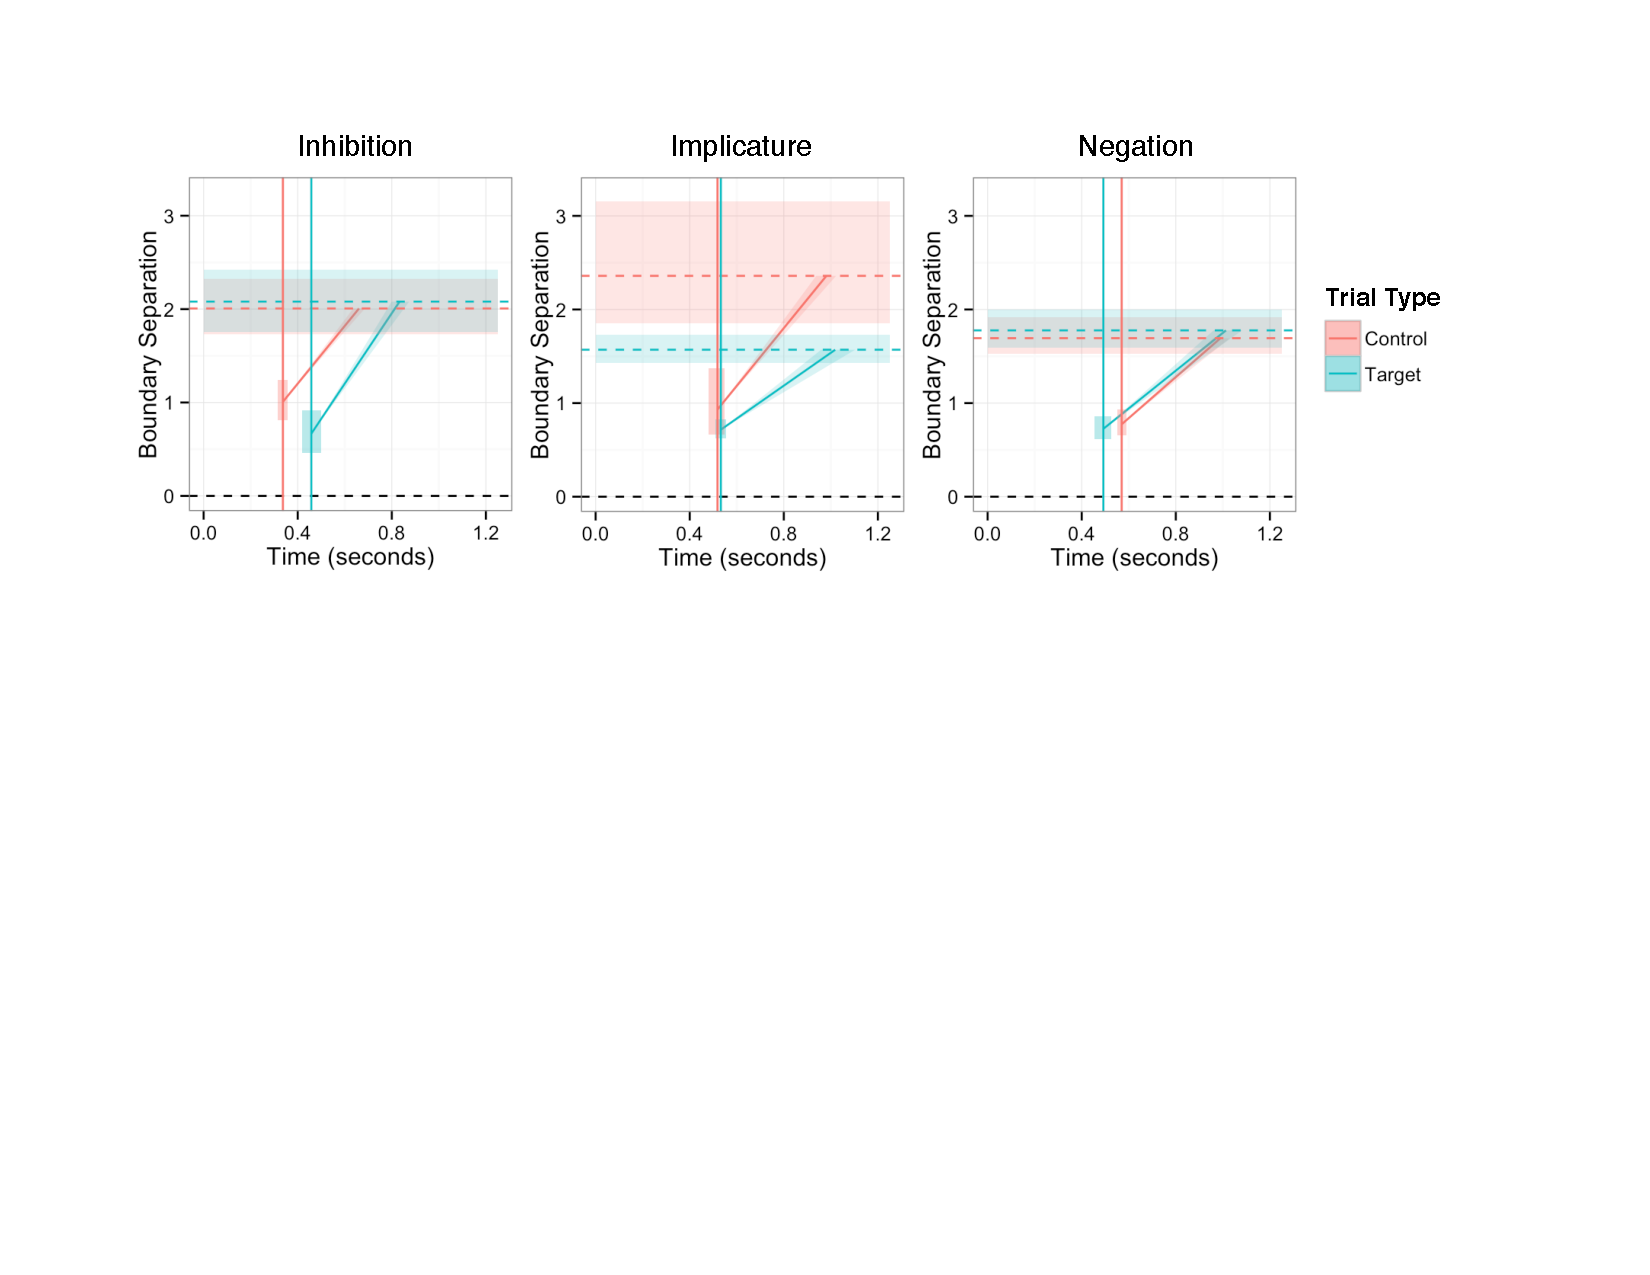
\includegraphics[width=6in]{figures/child_vis.pdf}
\caption{\label{fig:kids} Visualization of the drift diffusion process for 4-year-olds, 5-year-olds, and 6-year-olds across the three games.  Plotting conventions are the same as in Figure \ref{fig:adults}.}
\end{center} 
\end{figure*}

Next we explored developmental change in preschoolers between 4 and 7 years of age.  The decision process for each game across the three age groups is visualized in Figure \ref{fig:kids}.  For the inhibition and implicature games, children at all ages look similar to adults, with developmental change across the three age groups as children's decision process gets more adult-like.  For example, in the inhibition game, 4-year-olds are actually \emph{less} likely to show a bias towards the incorrect trial; this bias appears to get stronger by age 6.  In the implicatures game, children have a slower drift rate for target trials compared to control trials even at age 4, although this difference is not as large as it is for adults. The most striking difference between children and adults is in the negation game, where the drift rate for target trials is dramatically slower compared to control trials.  

To examine the reliability of our findings, we fit linear models to the data for each of the three games to explore how the interaction between trial type (control vs. target trials) and age group influences different parameters. For the bias parameter in the inhibition game, we see a significant positive interaction between age group and trial type for four-year-olds ($\beta = .16$, $p< .05$), indicating that for four-year-olds the bias parameter for target trials in the inhibition game is higher compared to adult participants.  There is no interaction between age group and trial type for five-year-olds ($\beta = .07$, $p = .26$), and a marginally significant \emph{negative} interaction between age group and trial type for six-year-olds ($\beta = -.10$, $p = .09$).  These results collectively suggest that while four year olds are \emph{less} biased towards the incorrect response on target trials compared to adults, by age six children are becoming more biased towards the incorrect response on target trials.  

For the drift rate parameter in the implicatures game, we found a main effect of age group, with a significantly slower drift rate overall for four-year-olds ($\beta = -1.98$, $p < .001$), five ($\beta = -1.46$, $p < .001$), and six-year-olds ($\beta = -1.33$, $p < .001$).  There was also a significant interaction between age group and trial type for four-year-olds ($\beta = 0.83$, $p <.01$), fives ($\beta = 0.71$, $p <.05$), and six-year-olds ($\beta = 0.72$, $p <.05$), indicating that the difference between drift rate for target vs. control trials is much smaller for children compared to adults.  We found the opposite pattern in the negation game: Although there was a similar main effect of age group, with four-year-olds showing significantly slower drift rates overall compared to adults ($\beta = -.92$, $p <.001$) and six-year-olds showing marginally slower drift rates compared to adults ($\beta = -.37$, $p = .07$), children at all age groups showed a \emph{greater} difference in drift rate between control and target trials compared to adults, as indicated by significant negative interactions between age group and trial type for all age groups (4-year-olds: $\beta = -.7-$, $p <.05$; 5-year-olds: $\beta = -1.00$, $p <.01$; 6-year-olds: $\beta = -.77$, $p <.01$).  

\subsubsection{General Developmental Change}
We can also use our data to look at overall changes in the decision process across age groups, regardless of the task that children were engaged in. Across all three games, children at all age groups had higher boundary separation parameters (4-year-olds: $\beta = 1.01$, $p <.001$; 5-year-olds: $\beta = 1.10$, $p <.001$; 6-year-olds: $\beta = .67$, $p <.001$) and longer non-decision times (4-year-olds: $\beta = .08$, $p <.001$; 5-year-olds: $\beta = .19$, $p <.001$; 6-year-olds: $\beta = .11$, $p <.001$) compared to adults, suggesting that children take longer to encode information and need more information to make a decision compared to adults.  Children also had significantly slower drift rates compared to adults (4-year-olds: $\beta = -1.39$, $p <.001$; 5-year-olds $\beta = -1.29$, $p <.001$; 6-year-olds: $\beta = -1.12$, $p <.001$), suggesting that children acquire evidence more slowly than adults.  These data replicate past findings from \citeA{ratcliff2012}, which found similar differences between adults and elementary-school aged children, with a much younger sample of children.  

To explore whether these parameters change significantly throughout these early years, we focused just on children's data and analyzed age group as a continuous variable.  This analysis revealed a significant increase in drift rate across these three years ($\beta = .14$, $p < .05$), as well as a significant decrease in separation bias ($\beta = -.15$, $p < .05$).  These findings indicate that the speed at which children accumulate evidence and the amount of information that children need to make a decision changes rapidly across early childhood.  

\section{General Discussion}

We designed a game with three similar phases to explore children's and adults' inhibitory control, implicature processing, and negation processing.  Our game was designed to explore similarities across the processing of these three games, all of which involved making a quick decision in response to a word and a picture.  Although we initially thought that all three of these tasks might involve some element of inhibitory control, we did not find any evidence in accuracy, reaction time, our our drift diffusion modeling to suggest that adults or children are biased towards the incorrect answer on implicature or negation tasks.  Our drift diffusion analysis shed light on the decision process that children and adults go through when responding to these tasks, and indicate that a great deal of developmental change takes place even throughout these few short years.

The drift diffusion model revealed two important findings in our data.  First, although the three phases of this game were nearly identical in appearance (i.e. using the same few trial images and labels, and the same basic instructions to select the correct picture), the decision process for adults to choose the correct picture was very different for each game.  The inhibition game was characterized by a bias towards the incorrect answer on target trials, for example, while the implicatures game was characterized by slower drift rates for target trials.  Second, children's difficulty on these tasks appears to be due to slow drift rates, especially for target trials.  Past work suggests that children typically have slower drift rates compared to adults \cite{ratcliff2012}, and our current work replicates that finding in our task.  The fact that children's drift rates were significantly slower for negation and implicature trials, however, suggests that children find it particularly difficult to process the relevant information about these stimuli above and beyond a generally slower processing speed for children compared to adults.

Another novel aspect of this work is the use of the drift diffusion model with such a young group of children.  Although some past work has explored children's information processing using the drift diffusion model \cite{ratcliff2012}, that work tested second graders at the youngest.  Here we expand on that work by examining a group of even younger children, and replicating their findings.  Our success using the drift diffusion model for such a young group of children opens doors for future work to explore information processing in young children in a number of similar domains.  \aen{sorry this is kind of weak, haha, I'm tired, will revise later} \ejy{here should we comment briefly about the advantage of DDM over traditional analysis, about how it revealed what we couldn't see from accuracy and rt alone?}

%\section{Acknowledgments}
%
%Bing Nursery School, CDM, Stephen Powell, Veronica, Rachel

\bibliographystyle{apacite}

\setlength{\bibleftmargin}{.125in}
\setlength{\bibindent}{-\bibleftmargin}

\bibliography{neginhib}


\end{document}
